\documentclass{sig-alternate-10pt}

\usepackage[breaklinks=true,colorlinks=true,plainpages=false,citecolor=blue,urlcolor=blue,filecolor=blue]{hyperref}
\usepackage{url}        % Not compatible with hyperref?
\usepackage{float}
\usepackage{graphicx}
\usepackage{amsmath}
\usepackage{color}
\usepackage{times}
\usepackage[sort]{natbib}
\usepackage{enumitem}
%\usepackage{subfigure}
\usepackage{verbatim}
\usepackage{xspace}
\usepackage{xfrac}
\usepackage{algorithmic} % must come after hyperref
\usepackage{algorithm}

\usepackage{listings}
\usepackage{microtype} %does typographical voodoo to get rid of most overfull
                       %boxes. Ideally requires pdfTeX 1.4+, going directly
                       %to pdf. Don't use a DVI workflow.
\usepackage{balance}   %\balance keywork has to be included in the last page that
                       % will not be balanced, in the first column.
\usepackage{datetime}
\usepackage{morefloats}

\usepackage{caption}
\usepackage{subcaption}

\DeclareMathVersion{mathchartertext}
\SetSymbolFont{letters}{normal}{OML}{mdbch}{m}{n}
\newcommand{\gchar}[1]{\mathversion{mathchartertext}$#1$\mathversion{normal}}

% Configure algorithmic and listings
\renewcommand{\algorithmicrequire}{\textit{Input:}}
\renewcommand{\algorithmicensure}{\textit{Output:}}
\lstset{%language=Python,
numberstyle=\footnotesize,
basicstyle=\ttfamily\scriptsize,
numbers=left,
stepnumber=1,
showstringspaces=false,
breaklines=true}

 \newcommand{\todo}[1]{\textcolor{blue}{\textbf{TODO:} #1}}
 \newcommand{\eric}[1]{\textcolor{red}{\textbf{Eric:} #1}}
 \newcommand{\aditya}[1]{\textcolor{red}{\textbf{Aditya:} #1}}
 \newcommand{\keqiang}[1]{\textcolor{red}{\textbf{Keqiang:} #1}}
\newcommand{\cut}[1]{}

%\newcommand{\todo}[1]{}
\newcommand{\jeff}[1]{}
\newcommand{\colin}[1]{}
\newcommand{\brent}[1]{}

\newcommand{\eg}{\emph{e.g.}\xspace}
\newcommand{\cf}{{cf.}\xspace}
\newcommand{\ie}{\emph{i.e.}\xspace}
\newcommand{\etal}{{et al.}\xspace}

\hyphenation{light-weight}
\hyphenation{meas-ure-ment}
\newcommand{\tightparagraph}[1]{\vspace{5pt}\noindent\textbf{#1}\ }

%ejr, adding per jitu's email
\setlength{\pdfpagewidth}{8.5in}
\setlength{\pdfpageheight}{11in}


%don't want date printed
\date{}


%\title{Presto: Distributed Flowcell Load Balancing at the \\ Datacenter Network Edge}

\title{Presto: Edge-based Load Balancing for Fast Datacenter Networks}
\author{Paper \#349, 12 pages + 1 page references}

\iffalse
\author{
{Keqiang He$^\dagger$ \hspace{0.2in} Eric Rozner$^\ast$ \hspace {0.2in} Kanak Agarwal$^\ast$}\\[.2cm]
{Wes Felter$^\ast$ \hspace{0.1in} John Carter$^\ast$ \hspace{0.1in} Aditya Akella$^\dagger$}\\\\
{\affaddr{$^\dagger$UW-Madison \hspace{0.15in} $^\ast$IBM Research }}\\\\
{\textcolor{red}{\normalsize Git-hash: \input{.git/ORIG_HEAD}}} \\
{\textcolor{red}{\normalsize \today, \currenttime}}
}
\fi

\newfont{\mycrnotice}{ptmr8t at 7pt}
\newfont{\myconfname}{ptmri8t at 7pt}
\let\crnotice\mycrnotice%
\let\confname\myconfname%


\clubpenalty=10000
\widowpenalty = 10000

\begin{document}

\maketitle

\begin{abstract}

A lot of recent work has been focusing on solving in network latency in datacenter networks. 
In this paper, we focus on a less explored topic \textemdash\xspace latency 
increase caused by rate limiters on the end-host. 
We show that latency can be increased by an order of magnitude 
by the rate limiters in cloud networks, 
and simply extending ECN into rate limiters is not sufficient. 
To this end, we propose two techniques \textemdash\xspace~\dem{} and~\spring{} to improve the performance of rate limiters. 
Our experiment results demonstrate that~\dem{} and~\spring{} enabled 
rate limiters can achieve high (and stable) throughput and low latency.

\iffalse
Bandwidth guarantee is an essential feature to satisfy tenants' QoS requirement in clouds. However, its token-buffer-based implementation is not compatible with other aspects of QoS, i.e., latency and packet loss. In this paper, we propose to \name, which guarantees bandwidth allocation, low latency and little packet loss. The main idea is to maintain a large token buffer to tolerate traffic burst and keep low buffer occupancy to obtain low queuing latency. The low occupancy is achieved by carefully adjust traversing flows' sending rate. We implement \name in two ways for different virtualized environments: 
(1) adjust flows' congestion window directly at token buffers according to instantaneous queue length, which suits VM-based clouds,  (2) enable ECN at token buffers and leverage DCTCP for congestion control at end points, which suits container-based clouds. We integrate \name into a widely used virtual switch \textemdash\xspace OVS, so that \name can be deployed without any changes to OS kernels. And our evaluation shows \wenfei{result}.

\fi

\end{abstract}



Cloud computing has been changing the way computing is conducted since a few years ago.
It is a rapidly growing business and many industry leaders
(\eg{}, Amazon~\cite{amazon-aws}, Google~\cite{google-compute}, 
IBM~\cite{ibm-softlayer,ibm-bluemix} and
Microsoft~\cite{microsoft-azure}) have embraced such a
business model and are deploying highly advanced cloud computing infrastructures.
Market analysis~\cite{cloud-market2020}
has predicted that the global cloud computing market will
reach \$270 billion by 2020. The success of cloud computing is
not accidental \textemdash\xspace it is rooted in many advantages that cloud computing offers
over traditional computing model. The most notable feature is that tenants
(customers) who rent the computing resources (e.g., CPUs, memory, storage, and network) can get equivalent computing power
with \emph{lower cost}. This is because the computing resources are shared among multiple users and
server consolidation and server virtualization improve the utilization
of the computing resources. Another key advantage cloud computing offers
is \emph{computing agility}. That means, tenants can rent as many computing
resources as they need and can grow or shrink the computing pool based on their demands 
in an elastic manner.
This feature is especially attractive for relatively smaller and
rapidly growing businesses.

Datacenter networks are important components in modern cloud computing infrastructures. 
High-performance cloud computing infrastructures require high-speed, low latency, scalable and 
highly robust datacenter networking solutions to support a massive amount of traffic. 
Cisco Global Cloud Index~\cite{cisco-predict} predicts that annual global datacenter IP traffic will 
reach 15.3 zettabytes (ZB) by 2020, which is 3 times large as 2015's (4.7 ZB). 
The tremendous growth of datacenter traffic drives the need for high-performance 
datacenter networking solutions. 

Datacenter network is a complicated system and it covers many 
aspects of computer networking, ranging from TCP congestion control algorithms to switch hardware design. 
In the past 10 years, datacenter networking technologies have been advanced significantly. 
For example, starting in 2009 - 2010, seminal works on datacenter network topology designs such as 
FatTree~\cite{fattree} and VL2~\cite{vl2} were published. 
These works proposed to use multi-stage Clos networks to 
scale out and support hundreds of thousands of servers in a single datacenter. 
Recently (in 2016), Microsoft published their congestion control solution for 
RDMA deployments in Azure networks~\cite{zhu2015congestion}. 
Despite these advances, there are still a lot of unsolved research challenges in datacenter networking.

In cloud computing, one of the key technology trends is software-defined datacenters. 
In particular, Software-defined Networking (SDN) technology has been widely 
applied in datacenter environments and has enhanced the agility and performance of datacenter networks.
In 2007, Casado et al presented a control plane and dataplane separation network architecture for 
Enterprise networks named Ethane~\cite{casado2007ethane}. 
In 2008, networking researchers, McKeown et al, argued that today's computer network 
devices (i.e., switch and routers) were commercialized black boxes, 
and it was increasingly harder for networking researchers to invent and test new networking 
techniques on existing networking devices. Their white paper~\cite{McKeown08} described the initial motivation 
for OpenFlow. Ethane and OpenFlow started the revolution of Software-defined Networking (SDN). 
Later on, an open source implementation of SDN-capable virtual switch, Open vSwitch (OVS)~\cite{Pfaff2015ovs}, was released. 
OVS is now maintained by VMware. 
OVS is widely deployed in cloud computing platforms to support network virtualization functionalities and 
meet SDN-style network management requirements.
OVS opened the door of software-define network edge (i.e., end-host network) in datacenter environments.
End-host networking covers many components, for example, TCP/IP stack, virtual switch, rate limiters and NIC hardware. 
In a datacenter network, all the servers (and hypervisors) are managed by a single entity 
(i.e., the cloud provider), therefore, there are a lof of opportunities for innovations, 
especially the innovations in end-host networking.

In this thesis, I will present our research works on improving datacenter networking performance. 
Performance here refers to network throughput, latency and packet loss etc. 
The major theme of this thesis is to leverage the intelligent software-defined network 
edge (i.e., end-host networking) to improve the performance for datacenter networks.
In the following of this chapter, I will briefly introduce three research projects I worked on 
during my PhD study, they are \textemdash\xspace edge-based traffic load balancing for 
datacenter networks, congestion control virtualization for multi-tenant clouds and 
low latency software rate limiters for cloud networks.

\section{Edge-based Traffic Load Balancing}

Modern datacenter networks are built with multi-stage Clos networks. 
A good example of such topologies is Google's Jupiter topology~\cite{singh2015jupiter}. 
A nice property of multi-stage Clos network is that there are tens to hundreds of 
network paths between any two servers in the datacenter. Path diversity is good for network 
reliability and traffic load balancing. The state-of-the-art approach of traffic load balancing 
is called Equal Cost Multipathing (ECMP). When a data packet arrives at a switch, 
there are many paths to the destination. The switch applies a hash function to several 
fields in the packet header, for example, source IP address, destination IP address, 
transport protocol, source port number and destination port number. Based on the hash value, 
the switch chooses one of the potential paths. ECMP can lead to traffic imbalance and 
does not work well in asymmetric networks, so Weighted Cost Multipathing (WCMP) was proposed~\cite{wcmp}.

Datacenter networks need to support various kinds of network traffic generated by 
a diverse set of applications and services running in the datacenters. For example, flows generated 
by search, email, query and remote procedure calls tend to be short and small, and we call such flows mice flows. 
On the other hand, flows generated by big data ingestion and data backup tend to be long and large, 
so we call such flows elephant flows. A classic problem of ECMP and WCMP is that if two elephant flows 
are hashed onto the same network path, then flows of both types suffer. First, elephant flows' throughputs are reduced. 
Second, mice flows suffer from head-of-line blocking issue and their latency can be increased to 
tens of milliseconds~\cite{alizadeh2012less}. 
Note that the baseline TCP RTT in the datacenter network environment is around 200 microseconds~\cite{he2016ac}. 
To solve this problem, we propose Presto. Presto has two novel components. At the sender side, 
we utilize the virtual switch (e.g., OVS) in the hypervisor to break elephant flows into small chunks 
called flowcells. A flowcell consists of several TCP segments and its maximum size is bounded to be the 
maximum TCP Segment Offload (TSO)~\cite{tcp-segment-offload} size, 
which is 64KB by default in Linux. In this way, packets of a mice flow whose size 
is smaller than or equal to 64KB always go through the same network path, so there is no packet reordering issue. 
For the flows that are larger than 64KB, packets may go through different paths and packet reordering 
issue may arise if the congestion level on different network paths is different. 
Therefore at the receiver side, we modify the Generic Receive Offload (GRO) functionality in the network stack to 
mask packet reordering for TCP. Because Presto eliminates elephant flow collision problem and 
masks packet reordering for large flows below TCP layer in GRO, the performance of 
traffic load balancing is greatly improved.
We will discuss the details of Presto in Chapter~\ref{thesis:chapter:presto}.


\section{Congestion Control Virtualization}
TCP congestion control is a long-lasting research problem in computer networking. 
The first TCP congestion control algorithm (TCP Reno) was proposed by Jacobson et al in 1988~\cite{jacobson1988congestion}. 
Since then a lot of research work has been done to optimize congestion control algorithms. 
Traditional congestion control algorithms are tuned for Internet use cases. However, 
datacenter network has its own unique characteristics. The most notable difference 
is that a datacenter network is owned by the single entity. Therefore, many of the deployment 
hurdles in Internet or Wide Area Networks (WANs) do not exist in datacenter environments. 
In 2010, Alizadeh et al published the seminal work on datacenter network congestion 
control \textemdash\xspace Datacenter TCP (aka DCTCP)~\cite{alizadeh2010data}. 
DCTCP utilizes ECN (Explicit Congestion Notification) in 
modern switches and adjusts TCP's congestion window based on the fraction of 
packets that are ECN-marked by the switches. DCTCP effectively reduces datacenter network latency, especially tail latency.

However, we still face a practical unsolved problem. Most of today's public clouds, e.g., 
Google Cloud Platform, Microsoft Azure and Amazon Web Services (AWS), are multi-tenant clouds. 
The computing resources (e.g., CPUs, memory, storage and network) are rented to 
tenants (i.e., customers) in the form of Virtual Machines (VMs). The practical problem is 
that cloud providers are not able to manage or configure the congestion control algorithms used 
by the VMs' TCP/IP stacks. Tenants can manage and configure their own TCP/IP stacks. So VM TCP congestion 
control algorithms can be outdated, inefficient or even misconfigured. Those outdated, inefficient or 
misconfigured TCP/IP stacks cause network congestion and fairness issues for the datacenter network. 
Therefore, we investigate if administrators can take control of a VM's
TCP congestion control algorithm without making changes
to the VM or network hardware. We propose \acdc{} TCP,
a scheme that exerts fine-grained control over arbitrary tenant
TCP stacks by enforcing per-flow congestion control in
the virtual switch (vSwitch). Our scheme is light-weight,
flexible, scalable and can police non-conforming flows. In
our evaluation the computational overhead of \acdc{} TCP
is less than one percentage point and we show implementing
an administrator-defined congestion control algorithm in the
vSwitch (i.e., DCTCP) closely tracks its native performance,
regardless of the VM's TCP stack.
We will discuss the details of \acdc{} TCP in Chapter~\ref{thesis:chapter:acdctcp}.

\section{Low Latency Software Rate Limiters}
The ability to create bandwidth allocations is an indispensable feature
of multi-tenant clouds.  Bandwidth allocations can be used to provide
bandwidth reservations to a tenant or to guarantee that network
bandwidth is fairly shared between multiple competing
tenants~\cite{shieh2011sharing,jeyakumar2013eyeq,rodrigues2011gatekeeper}.
Bandwidth allocations are often implemented with \textit{software rate
limiters} running in the hypervisor or operating system
of the end-hosts attached to the network (e.g., Linux Hierarchical Token
Bucket, aka HTB).  This is because software rate limiters are flexible
and scalable.
Unfortunately, typical software rate limiters (e.g., HTB) also increase
network latency by adding an additional layer of queuing for packets.
To be able to absorb bursts of incoming packets while also ensuring that
network traffic does not exceed the configured rate, rate limiters
maintain a queue of outstanding packets and control the speed at which
packets are dequeued into the network.  This queuing introduces
additional network latency.  For example, in our experiments, we find
that software rate limiting (HTB) increases latency by 1-3 milliseconds
across a range of different environment settings. This increase in
latency is about an order of magnitude higher than the base latency of
the network (200 microseconds). In multi-tenant clouds, this additional queuing
latency can increase flow completion times, leading to possible
service-level agreement (SLA) violations~\cite{wilson2011better}.

Inspired by recent work that reduces queuing delay for in-network
devices like switches ~\cite{alizadeh2010data,he2016ac,mittal2015timely,zhu2015congestion}, we explore how to
use a congestion-control-based approach to address the latency issues
associated with using software rate limiters.  As a promising first
step, we find that the existing datacenter congestion control protocol
DCTCP~\cite{alizadeh2010data} can be used to reduce the latency incurred
by rate limiters. Unfortunately, we find that a straightforward
application of DCTCP (we call it DCTCP+ECN) to software rate limiters also hurts throughput because of 
two problems unique to end-host networking. First, different from hardware switches in the
network, end-hosts process TCP segments instead of MTU-sized packets.
TCP Segmentation Offload (TSO)~\cite{tcp-segment-offload} is an
optimization technique that is widely used in modern operating systems
to reduce CPU overhead for fast speed networks. Because Linux has
difficult driving 10Gbps (and beyond) line-rates when TSO is not
enabled, Linux uses a TSO size of 64KB by default. That means that
marking the ECN bit in one 64KB segment causes 44 consecutive MTU-sized
packets to have the ECN bit marked. This is because the ECN bits in the
segment header are copied into each packet by the NIC. Oppositely, if a
TCP segment is not marked, none of the packets in this segment is
marked. This kind of coarse-grained segment-level marking leads to an
inaccurate estimation of congestion level which consequently leads to
throughput oscillation.
The second problem with DCTCP+ECN is that the ECN mark takes one
round-trip time (RTT) to get back to the source.  Because of this, the
congestion window computation at the source uses a stale value from one
RTT ago. As a result, congestion cannot be detected at early stage, and
the congestion level would be exacerbated during this one-RTT delay.
To solve the problems, we present two techniques \textemdash\xspace~\dem{} and ~\spring{}.
~\dem{} directly sets TCP ACK's TCP ECE (Echo-Echo) bit based on real time rate limiter queue length information.
In this way, congestion control loop latency is reduced to almost 0. Also coarse-grained segment-level marking is avoided.
~\spring{} runs a queue-length-based congestion control algorithm and enforces congestion control decisions via modifying
the~\rwnd{} field in the TCP header. Similar to~\dem{},~\spring{} also avoids the two shortcomings of DCTCP+ECN. 
Compared with~\dem{},~\spring{}
is more generic and deployable because it does not rely on ECN support.
We will discuss the details of low latency software rate limiters in Chapter~\ref{thesis:chapter:rate_limiter}.

\section{Summary of Contributions and Overview}

The contributions of this dissertation are summarized in the following. 
This section also serves as an outline for the rest of this dissertation.

\begin{itemize}
\item Edge-based Datacenter Traffic Load Balancing. We propose two novel techniques. 
The first is to utilize the virtual switch (e.g., OVS) in the hypervisor to chunk flows into bounded-sized flowcells. 
The second is to leverage the Generic Receive Offload (GRO) functionality in the networking stack to 
mask packet reordering for TCP layer. To the best of our knowledge, we are the first to 
present these two techniques in the literature. Based on these two techniques, we build a datacenter 
traffic load balancing system called Presto and evaluate its performance on a real 10G testbed. 
Our experiment results demonstrate that Presto improves network performance significantly. 
We will cover the details of Presto in Chapter~\ref{thesis:chapter:presto}.
 
\item Congestion Control Virtualization for Datacenter Networks. 
We propose AC/DC TCP, a technique that utilizes the virtual switch in the hypervisor 
to provide congestion control virtualization for multi-tenant clouds. 
To the best of our knowledge, we are one of the first two research teams\footnote{The other team is from 
Stanford, VMware and Israel Institute of Technology~\cite{vcc}; we invented the same technique independently.} in the world to 
propose the congestion control virtualization technique for cloud networks. 
We validate its feasibility on a real testbed and demonstrate that it provides similar 
performance as the intended congestion control algorithm. Chapter~\ref{thesis:chapter:acdctcp} covers the details of AC/DC TCP.
 
\item Low latency Software Rate Limiters. Rate limiters are important 
components for multi-tenant clouds. We conduct experiments to show that network latency 
can be increased by an order of magnitude by software rate limiters. We extend ECN into rate 
limiter queues and apply DCTCP to reduce latency. However, we find such a straightforward 
solution causes TCP throughput oscillation. We identify the reasons and propose 
two techniques (i.e.,~\dem{} and ~\spring{}) to address of shortcoming of the 
straightforward solution. Our experiments demonstrate that~\dem{} and ~\spring{} enable 
low latency software rate limiters. The research work on software rate limiters is 
discussed in Chapter~\ref{thesis:chapter:rate_limiter}.

\item Related Work. We present the related work of this dissertation in Chapter~\ref{thesis:chapter:related}. 
It covers related work in the following categories: datacenter network traffic load balancing, 
reducing tail latency, handling packet reordering, congestion control for datacenter networks, 
bandwidth allocation and rate limiters for multi-tenant clouds.

\item Conclusion and Future Work. We conclude this dissertation in Chapter~\ref{thesis:chapter:conclusion}. 
We believe that the techniques and mechanisms presented in this dissertation 
will be valuable to the computer networking research community and industry. 
Finally, we discuss several future research topics in datacenter networking area. 
\end{itemize}



\section{Background and Motivation}
\label{background}
This section first gives a brief background of congestion 
control in the datacenter. Then the motivation for moving congestion
control into the vSwitch is presented. Finally,~\acdc{} is contrasted from a class of related bandwidth
allocation schemes.

\subsection{Datacenter Transport}
\label{ss:dct}
Today's datacenters host applications such as search,
advertising, analytics and retail that require high bandwidth and low latency.
%Large tail latencies often violate the tight timing constraints required by SLAs at scale, and
%have been shown to impact customer experience, result in
%revenue loss~\cite{alizadeh2011data,dean2013tail}, and degrade application performance~\cite{jang2015silo,qjump}.
%Tail latencies are often caused by network congestion.
%The latency of traversing a single switch, NIC and OS network stack is 10--30$\mu$s,
%2.5--32$\mu$s and 15$\mu$s respectively, but a congested port
%on a network switch can consume significant shared memory, causing orders-of-magnitude
%higer latency~\cite{rumble2011s}.
Network congestion, caused by imperfect load balancing~\cite{al2010hedera},
network upgrades or failures, can adversely impact these services. Unfortunately, congestion is
not rare in datacenters. For example, recently Google reported 
congestion-based drops were observed when network utilization approached 25\%~\cite{singh2015jupiter}.
Other studies have shown high variance and substantial increase in the 99.9$^{th}$ percentile latency
for round-trip times in today's datacenters~\cite{wang2010impact,mogul2015inferring}. 
Large tail latencies impact customer experience, result in
revenue loss~\cite{alizadeh2011data,dean2013tail}, and degrade application performance~\cite{jang2015silo,qjump}.
Therefore, significant motivation exists to reduce congestion in datacenter fabrics.

%Studies have shown that while CUBIC can achieve
%high bandwidth, it does so at the cost of aggressively filling up the switch buffers in the network.
TCP's congestion control algorithm is
known to significantly impact network performance.
As a result, datacenter TCP performance has been widely
studied and many new protocols have been proposed~\cite{alizadeh2011data, stephens2014practical, wu2010ictcp,
mittal2015timely, jose2015high}. Specifically, DCTCP~\cite{alizadeh2011data} adjusts a TCP sender's rate based on the fraction of packets experiencing congestion. In DCTCP,
the switches are configured to mark packets with an ECN bit when their queue lengths exceed a threshold. By proportionally
adjusting the rate of the sender based on the fraction of ECN bits received, DCTCP can keep queue lengths low, 
maintain high throughput, and increase fairness and stability over traditional schemes~\cite{alizadeh2011data,judd2015nsdi}.
\crs{For these reasons, we implement DCTCP as the vSwitch congestion control algorithm in~\acdc{}.}

\subsection{Benefits of~\acdc{}}
%Rather than proposing a new datacenter congestion control algorithm, this work investigates
%if congestion control can be moved to the vSwitch.
Allowing administrators to enforce an optimized congestion control without
changing the VM is the first major benefit of our scheme.
This is an important criteria in untrusted public cloud environments or simply in cases where servers cannot be updated
due to a dependence on a specific OS or library.~\cite{judd2015nsdi}


\begin{figure}[!t]
        \centering
        \begin{subfigure}[b]{0.45\textwidth}
                \centering
		%max min mean median
                %\includegraphics[width=\textwidth]{acdctcp/figures/tput_fairness/default_5CC_tput.pdf}
                %5 CCs
		\includegraphics[width=\textwidth]{acdctcp/figures/tput_fairness/default_5CC_tput_detail.pdf}
		\caption{5 different CCs.}
                \label{unfairness_5CC}
        \end{subfigure}
        \begin{subfigure}[b]{0.45\textwidth}
                \centering
                \includegraphics[width=\textwidth]{acdctcp/figures/tput_fairness/default_all_cubic_tput.pdf}
                \caption{All CUBIC.}
                \label{unfairness_all_cubic}
        \end{subfigure}
%        \begin{subfigure}[b]{0.24\textwidth}
%                \centering
%                \includegraphics[width=\textwidth]{acdctcp/figures/tput_fairness/liquid_5CC_tput.pdf}
%                \caption{5 different CCs with \acdc{}.}
%                \label{fairness_5CC_with_ours}
%        \end{subfigure}
%        \begin{subfigure}[b]{0.24\textwidth}
%                \centering
%                \includegraphics[width=\textwidth]{acdctcp/figures/tput_fairness/ecn_all_dctcp_tput.pdf}
%                \caption{All DCTCP.}
%                \label{fairness_5CC_with_dctcp}
%        \end{subfigure}
        \caption{Different congestion controls lead to unfairness.}
        \label{tput_unfair}
\end{figure}

The next benefit is~\acdc{} allows for {\em uniform}
congestion control to be implemented throughout the datacenter.
Unfairness arises when stacks are handled differently in the fabric or when conservative and aggressive
stacks coexist. Studies have shown ECN-capable and ECN-incapable flows do not exist gracefully on the
same fabric because packets belonging to ECN-incapable flows encounter severe packet drops when their packets
exceed queue thresholds~\cite{wu2012tuning,judd2015nsdi}. %Ideally, tenants shouldn't suffer based on such a simple configuration issue.
%~\eric{Do we have an argument that clients should be able to port their VMs to the cloud without making any changes
%or worrying about the low-level network details of the cloud provider?}
Additionally, stacks with different congestion control algorithms may not share the same fabric fairly.
For example, Figure~\ref{tput_unfair} shows the performance of five different TCP flows on the topology in
Figure~\ref{dumbbell_topology}. Each flow selects a congestion control algorithm available in Linux:
CUBIC~\cite{ha2008cubic}, Illinois~\cite{liu2008tcp}, HighSpeed~\cite{RFC3649},
New Reno~\cite{RFC3782} and Vegas~\cite{Brakmo1994}.
Figure~\ref{unfairness_5CC} shows aggressive stacks such as Illinois and HighSpeed
achieve higher bandwidth and thus fairness is worse than all flows using the
same stack (Figure~\ref{unfairness_all_cubic}). 
%A tenant should not be able
%to unfairly obtain higher bandwidth by simply changing its congestion control.

Another benefit of~\acdc{} is it allows for different congestion control algorithms to be assigned on
a per-flow basis. %Today, TCP congestion control is configured at an OS-level, so all of an OS's flows are forced to use the same congestion control algorithm.
A vSwitch-based approach can assign WAN flows to a congestion control algorithm that optimizes WAN performance~\cite{tan2006compound,flach2013reducing} and
datacenter flows to one that optimizes datacenter performance, even if these flows originate from the same VM (\eg{}, a webserver).
%This severely limits flexibility and forces tenants to optimize the performance of a subset of its flows. For example, a web server may choose a TCP stack to optimize
%WAN performance~\cite{tan2006compound,flach2013reducing} at the cost of harming back-end performance within the datacenter.~\eric{still need to clean}
Additionally, as shown in \cref{ss:cc-qos}, a flexible congestion control algorithm can provide relative bandwidth allocations to flows.
This is useful when tenants or administrators want to prioritize flows assigned to the same quality-of-service class.
In short, adjusting congestion control algorithms on a per-flow basis allows for 
enhanced flexibility and performance.
%As studies have shown that TCP can be optimized for datacenters~\cite{alizadeh2011data, stephens2014practical, wu2010ictcp,
%mittal2015timely, jose2015high}, WAN environments~\keqiang{cite Compound TCP?}, and even
%~\eric{one more example, wireless/60Ghz/free-space optics?}, selecting a per-flow TCP stack has the potential to
%enhance network performance. By moving congestion control to the vSwitch, administrators can assign a specific congestion control
%algorithm to each flow, optimizing the network performance of its clients in a seamless manner.~\eric{Also add QoS-based CC
%stuff here, since we have something.}

Finally, congestion control is not difficult to port. While the entire TCP stack may seem complicated and prone to high overhead,
the congestion control aspect of TCP is relatively light-weight and simple to implement. Indeed, studies
show most TCP overhead comes from buffer management~\cite{optimize-tcp-receive}, and
in our evaluation the computational overhead of~\acdc{} is less than one percentage point.
Porting is also made easy because congestion control implementations in Linux
are modular: DCTCP's congestion control resides in {\tt tcp\_dctcp.c} and is only about 350 lines of code. Given
the simplicity of congestion control, it is not hard to move its functionality to another
layer.
%~\crs{Furthermore,~\acdc{} does not rate limit or buffer packets, and our
%benchmarks show the computational overhead of~\acdc{} is less than one percentage point.}


\subsection{Tenant-Level Bandwidth Allocation}
%In addition to controlling congestion, public cloud administrators have to find ways to
%isolate the performance of different tenants and applications. 
\crs{While~\acdc{} enforces congestion control, transport layer schemes do not
provide fair bandwidth allocation among tenants because
a tenant with more concurrent flows can obtain
a higher share of bandwidth.
%The situation is further worsened by UDP flows since they are not subjected to any transport
%level congestion control.
In order to provide performance isolation in the network, datacenter operators can implement
a variety of bandwidth allocation schemes by either guaranteeing or proportionally
allocating bandwidth for tenants~\cite{rodrigues2011gatekeeper,Ballani2011oktopus,jeyakumar2013eyeq,shieh2011sharing,
Guo2010Secondnet,Popa2012Faircloud,Xie2012Proteus,Lam2012NetShare,jang2015silo}. 
%Simple static rate limiters enforced on many default public cloud images dictate an upper-bound on the bandwidth available
%to different classes of VMs.
% Congestion can occur when the cumulative bandwidth from a set of
%senders exceeds the bandwidth of a network link (incast is a special case). Consider the topology in Figure~\ref{dumbbell_topology},  
%with 5 flows traversing a bottleneck 10 Gbps link. Even in the case of a "perfect" allocation, where each flow is statically limited to 10 Gbps/5 flows = 2 Gbps,
%the latency caused by queueing heavily depends on the deployed TCP stack. We show this in Figure~\eric{cubic-fill}.
%CUBIC~\cite{ha2008cubic}, the default TCP congestion control algorithm in Linux, will aggressively fill
%the buffer of the congested output port, causing latencies to significantly increase. DCTCP, however, is able
%to keep buffers low~\cite{alizadeh2011data}, allowing for a queueing latency that is an order of magnitude lower than CUBIC's. These differences exist despite the fact
%that each scheme is able to achieve the same throughput over the congested link (Section~\ref{results}~\eric{Table 1}).
%Note that in Figure~\ref{cubic-fill}, DCTCP is run in the absence of a static rate limiter, meaning that it is effective
%in mitigating congestion's impact on latency. 
Some of these schemes share high-level architectural similarities to~\acdc{}.}
For example, EyeQ~\cite{jeyakumar2013eyeq} 
%provides a single dedicated switch abstraction for tenant VMs and 
handles bandwidth allocation at
the edge with a work-conserving distributed bandwidth arbitration scheme. It enforces
rate limits at senders based on feedback generated by receivers. Similarly, Seawall~\cite{shieh2011sharing}
provides proportional bandwidth allocation to a VM or application by forcing all
traffic through a congestion-controlled tunnel configured through weights and endpoint feedback.


The fundamental difference between these schemes and our approach is the design
goals determine the granularity on which they operate. 
Performance isolation schemes generally focus on {\em bandwidth allocation on a VM-level} and
are not sufficient to relieve the network of congestion because they do not
operate on flow-level granularity. 
For example, the single switch abstraction
in EyeQ~\cite{jeyakumar2013eyeq} and Gatekeeper~\cite{rodrigues2011gatekeeper} explicitly assumes a congestion-free 
fabric for optimal bandwidth allocation between pairs of VMs. This abstraction doesn't hold in multi-pathed
topologies when failure, traffic patterns or ECMP hash collisions~\cite{al2010hedera} cause congestion in the core.
Communication between a pair of VMs may consist of
multiple flows, each of which may traverse a distinct path. Therefore,
enforcing rate limits on a VM-to-VM level is too coarse-grained to determine how specific flows should adapt in
order to mitigate the impact of congestion on their paths. Furthermore, a scheme like Seawall~\cite{shieh2011sharing}
cannot be easily applied to flow-level granularity because
its rate limiters are unlikely to scale in the number of flows at high networking speeds~\cite{radhakrishnan2014senic}
and its allocation scheme does not run at fine-grained round-trip
timescales required for effective congestion control. Additionally, Seawall violates our design
principle by requiring VM modifications to implement congestion-controlled tunnels.

%Three bandwidth allocation schemes, EyeQ~\cite{jeyakumar2013eyeq}, Gatekeeper~\cite{rodrigues2011gatekeeper} and Seawall~\cite{shieh2011sharing}
%use congestion control techniques to provide bandwidth guarentees. At a high-level, these schemes employ
%VM-to-VM tunnels that partition bandwidth at the network edge (EyeQ) or proportionally allocate bandwidth
%over network links (Seawall). In addition, both EyeQ and Seawall are designed to adapt to network congestion
%by analyzing the fraction of packets marked with ECN bits to adjust the rates imposed on the VM-to-VM tunnels. 
%VM-to-VM tunnels are not fine-grained enough to effective mitigate queueing latencies caused by congestion.
%For example, datacenter topologies typically contain multiple paths from a source to a destination. Therefore,
%if a VM has multiple flows to another VM, those flows may take seperate paths (thanks to ECMP). By combining all flows
%over a single logical VM-to-VM tunnel, the proportion of packets experiencing congestion gets muddled. Flows that
%are not experiencing any congestion get their rates reduced unneccesarrily. Flows that are experiencing congestion
%do not reduce their rates fast enough.~\eric{i know this needs work} 

%\eric{Seawall talk mentioned O($10^5$) new tasks per minute. Can we make something more concrete above?}


\begin{figure}[!t]
        \centering
  \includegraphics[width=0.7\textwidth]{acdctcp/figures/motivation/motivation_2Gbps_cubic_rl_dctcp_sockperf.pdf}
        \caption{CDF of RTTs showing CUBIC fills buffers.}
        \label{cubic-fill}
\end{figure}
%\subsection{Bandwidth Allocation with Transport Control}
%In fact, bandwidth allocation schemes attempt to provide tenant level performance isolation
%regardless of the tenant transport stack and protocol, even though the stack has a large impact on congestion. 
~\crs{The above points are not intended to criticize any given work, but rather support the argument that
it is important for a cloud provider to enforce {\em both} congestion control and bandwidth allocation.
Congestion control can ensure low latency and high utilization, and
bandwidth allocation can provide tenant-level fairness.}
Bandwidth allocation schemes alone are insufficient to mitigate congestion because certain TCP stacks aggressively
fill switch buffers. Consider a simple example where five flows send simultaneously
on the 10 Gbps topology in Figure~\ref{dumbbell_topology}. Even when the bandwidth is allocated "perfectly"
at 2 Gbps per flow, CUBIC saturates the output port's buffer and leads to inflated round-trip times (RTTs) for traffic
sharing the same link.
%~\footnote{Note the servers are not over-subscribed in this scenario, so even
%bounding rate limiters to 10 Gbps may be deemed satisfactory by some edge-based bandwidth allocation schemes.}. 
Figure~\ref{cubic-fill} shows these RTTs for CUBIC and also DCTCP, 
which is able to keep queueing latencies, and thus RTTs, low even though no rate limiting was applied.
Therefore, it is important for cloud providers to exercise a desired congestion
control.

In summary, our vision regards enforcing tenant congestion control and bandwidth allocation as {\em complimentary} and we claim 
an administrator should be able to
combine any congestion control (\eg{}, DCTCP) with any bandwidth allocation scheme (\eg{}, EyeQ). 
Flow-level congestion control and tenant performance isolation need not be solved by the same scheme,
so~\acdc{}'s design goal is to be modular in nature so it can co-exist with any bandwidth allocation scheme
and its associated rate limiter (and also in the absence of both). 
%To the best of our knowledge,~\acdc{} is the first work that advocates moving flow-level transport congestion control
%out of the VM and into the hypervisor.~\eric{keep?}

%~\eric{is this fair in respect to seawall? and what about NICs that support full TCP offload?}
%A key design goal of~\acdc{} is for it to be modular in nature so it can co-exist with any bandwidth allocation scheme 
%and its associated rate-limiter (and also in the absence of both).
%In order to achieve this goal,~\acdc{} satisfies a variety of constraints. First, it is
%computationally light-weight in order to minimize the overhead of its adoption. Second,
%it doesn't require any changes to VMs or network hardware so it can be deployed in
%current and future networks. Third, our scheme works in the absence of specific topology
%information and works over arbitrary topologies. Fourth, it does not require
%any information about tenant traffic patterns or require specific VM placement or admission
%mechanisms.
%

\section{Design}
\label{rate-limiter:sec:design}

\subsection{Direct ECE Marking}
\begin{algorithm}[!t]
\caption{Pseudo-code of Direct ECE Marking Algorithm}
\label{alg:algorithm1}
\begin{algorithmic}[1]
\FOR{each incoming TCP ACK p}
\STATE q $\leftarrow$ rate\_limiter\_queue(p)
\IF{len(q) $>$ {\emph {K}}}
\STATE tcp(p).ece $\leftarrow$ 1
\ENDIF
\ENDFOR
\end{algorithmic}
\end{algorithm}

In this subsection, we introduce a technique called Direct ECE Marking (DEM). 
DEM requires that VMs and containers are configured with DCTCP congestion control algorithm. 
In~\dem{}, we monitor rate limiter queue occupancy and process each incoming TCP ACK. 
If the current rate limiter queue occupancy is above a threshold $K$, 
we directly set the ACK's TCP ECE (ECN Echo) bit to 1.
To get the correct rate limiter queue occupancy for the TCP ACK, we need to inspect the TCP ACK and
determine which queue the incoming TCP ACK's data packet belongs to. In other words, we need to 
determine the queue that this TCP ACK's reverse flow goes to.
The pseudo-code of~\dem{} is presented in Algorithm~\ref{alg:algorithm1}.~\dem{} can be
implemented in the virtual switch (e.g., OVS) in the hypervisor. OVS rate limiters directly call
the Linux HTB implementation so it can get the rate limiter queue information. Also, OVS processes all the packets
so it can inspect and modify all the incoming TCP ACKs. 

The difference between~\dem{} 
and existing ECN marking schemes is that it directly marks TCP ECE bit based on 
current queue occupancy instead of the queue occupancy one TCP RTT ago if using the existing ECN marking schemes.
Therefore, congestion control actions depend on real-time queueing information and control loop latency 
is reduced to almost 0. Control loop latency is the time it takes to forward the TCP ACK from the 
virtual switch to the VM or container. In this way, ``in network'' latency does not cause 
side-effects for end-host congestion control. Note that if we perform ECN marking on the outgoing path, then 
congestion control loop latency can be very large (e.g., RTT of the flows to remote clients is tens of ms).
Besides reducing control loop latency,~\dem{} also avoids coarse-grained segment-level ECN marking, 
which leads to inaccurate congestion level estimation, as we discussed before.
Therefore,~\dem{} makes rate limiter congestion control more timely and effective.

DEM only turns TCP ECE bit from 0 to 1, it never does the opposite. 
If congestion happens both in the rate 
limiter on the end-host and in the switch(es) on the network path, Then TCP ECE bit is always 1. 
If congestion only happens
in the rate limiter, then~\dem{} turns TCP ECE bit from 0 to 1. 
If congestion only happens in the network (i.e., in the switches), then TCP ECE is kept as 1.
If neither network switches nor the rate limiter is congested, then TCP ECE is always 0.
So~\dem{} does not affect the correctness of end-to-end
congestion control and is complementary with ``in network'' congestion control schemes.

\subsection{~\spring{}}

\begin{algorithm}[!t]
\caption{Pseudo-code of~\spring{} Algorithm}
\label{alg:algorithm3}
\begin{algorithmic}[1]
\FOR{each packet p}
\STATE q $\leftarrow$ rate\_limiter\_queue(p)
\STATE current\_qlen $\leftarrow$ len(q)
\STATE new\_gradient $\leftarrow$ current\_qlen -- q.prev\_qlen
\STATE q.prev\_qlen $\leftarrow$ current\_qlen
\STATE q.gradient $\leftarrow$ (1 -- $\alpha$)*q.gradient + $\alpha$*new\_gradient
\STATE q.normalized\_gradient $\leftarrow$ q.gradient / {\emph {K1}}
\IF{p is an incoming TCP ACK}
\STATE f $\leftarrow$ getReverseFlow(p)
\IF {current\_qlen $<$ {\emph {K1}}}
\STATE f.rwnd $\leftarrow$ f.rwnd + MSS
\ELSIF {current\_qlen $>$ {\emph {K2}}}
\STATE f.ssthresh $\leftarrow$ f.rwnd
\STATE f.rwnd $\leftarrow$ f.rwnd*(1 -- $\beta$*(1 -- $\frac{K2}{current\_qlen}$))
\STATE f.rwnd $\leftarrow$ max(f.rwnd, MSS)
\ELSIF {q.gradient $\le$ 0}
\STATE f.rwnd $\leftarrow$ f.rwnd + MSS
\ELSE
\STATE f.rwnd $\leftarrow$ f.rwnd*(1 -- $\beta$*q.normalized\_gradient)
\STATE f.rwnd $\leftarrow$ max(f.rwnd, MSS)
\ENDIF
\ENDIF
\ENDFOR
\end{algorithmic}
\end{algorithm}

DEM has two limitations. First is that it relies on 
DCTCP transport in VMs and containers. For containers, cloud administrators are able to configure
server's congestion control algorithm to DCTCP. So such an assumption is reasonable. 
However, for VMs, tenants have the flexibility to tune their congestion control settings.
Therefore, assuming that every VM uses DCTCP as the congestion control algorithm is not realistic in practice.
Second,~\dem{} needs ECN support in the network. As mentioned before, 
ECN is not widely supported in WAN traffic~\cite{kuhlewind2013state}.
To address the limitations and make our solution more generic, we present~\spring{} (shown in Algorithm~\ref{alg:algorithm3}).

~\spring{} modifies TCP ACK's receiver's 
advertised window size (also known as~\rwnd{}) to enforce congestion control~\cite{he2016ac,vcc}.
It uses real-time rate limiter queue length as congestion control signal and 
a TIMELY-like~\cite{mittal2015timely} congestion control law.
For each packet, 
we get its corresponding rate limiter queue length.
If the packet is outgoing, we get the length of the queue that the packet is to be enqueued.
If the packet is an incoming TCP ACK, we get the length of the queue that 
its reverse flow goes to (TCP is bidirectional).  
We maintain a gradient for the rate limiter queue length using 
Exponentially Weighted Moving Average (EWMA) (line 2--6). 
We set two thresholds, $K1$ and $K2$ ($K1 < K2$). The queue length gradient is normalized by dividing it using $K1$ (line 7).
Note that gradient is a per-queue defined parameter.
If the processed packet is an incoming TCP ACK, we first need to get its reverse 
flow (i.e., the TCP ACK's corresponding data packet flow). Then, 
we manage a running RWND for each flow based on a TIMELY-like congestion control law 
(line 10-- line 20). There are 4 cases: 
if the current rate limiter queue length is smaller than $K1$, that means this is no congestion, so we 
increase the flow's RWND by one MSS (Maximum Segment Size). If the current rate limiter queue length is larger
than $K2$, that means congestion happens in the rate limiter queue, so we multiplicatively decrease the RWND. 
If the current rate limiter queue length is between $K1$ and $K2$, we check the gradient of rate limiter queue occupancy.
If the gradient is smaller than or equal to 0, that means the queue is being drained or its size is not increasing, we 
increase RWND by one MSS. Otherwise, we multiplicatively decrease the RWND based on the normalized gradient.

Note that TIMELY~\cite{mittal2015timely} is a rate-based congestion control algorithm while~\spring{} is a window-based.
TIMELY uses accurate latency measurement provided by the NIC while~\spring{} performs congestion control based on 
real-time rate limiter queue length because ~\spring{} checks the rate limiter queue length when receiving 
incoming TCP ACKs. Because congestion control decisions are enforced via modifying RWND field in TCP ACK headers,~\spring{} has the following good properties: 
1) the solution does not relies on DCTCP transport in VMs and ECN support in the network, 
so it is generic and can support not only east-west traffic (i.e., intra-datacenter traffic) but also north-south traffic
(i.e., inter-datacenter traffic and traffic between cloud and clients). 
2) the solution avoids coarse-grained segment-level ECN marking and its control loop latency is almost 0, so congestion control
is more effective compared with the strawman solution---DCTCP in VMs/containers and ECN marking in rate limiter queues.  

\subsection{Remarks}
Both~\dem{} and~\spring{} avoid long and unpredictable congestion control loop latency and avoid throughput oscillation due to 
coarse-grained segment-level ECN marking.~\dem{} relies on ECN support in the network and DCTCP transports configured in
the end-points. Compared with~\dem{},~\spring{} is a more generic solution.~\dem{} and~\spring{} share the same limitation, that is
they do not support IPSec (because they need to modify TCP header). However, SSL/TLS is supported. 
Furthermore,~\spring{} needs to maintain per-flow information in the hypervisor. 
Maintaining per-flow information in switches is conventionally considered to be challenging.
In~\spring{} we only need to maintain the information of the connections from the VMs/Containers running on the end-host. 
Also, recent advances like OVS ConnTrack~\cite{ovs-conntrack} has made connection tracking on the end-host more effective.


\section{Implementation}
\label{sec:implementation} \mylabel{sec:implementation}

\section{Microbenchmarks}
\label{sec:micro}

We first evaluate the effectiveness of Presto over a series of microbenchmarks: %. Using 
%canonical topologies, we investigate 
(i) Presto's effectiveness in preventing the small segment
flooding problem and reordering, (ii) Presto's CPU overhead, (iii) Presto's ability to scale
to multiple paths, (iv) Presto's ability to handle congestion, (v) comparison to flowlet
switching, and (vi) comparison to local, per-hop load balancing.

%%%%%micro test - scalability and congestion test topology
\begin{figure}[t]
        \centering
	\begin{subfigure}[b]{0.225\textwidth}
        	\centering
  		\includegraphics[width=\textwidth]{presto/figures/micro_test_topology/micro_scalabilitytest_topology_refined.pdf}
        	\caption{}
		\label{micro_scalability_topology}
	\end{subfigure}
	\begin{subfigure}[b]{0.225\textwidth}
                \centering
		\includegraphics[width=\textwidth]{presto/figures/micro_test_topology/micro_congestiontest_topology_refined.pdf}
        	\caption{}
		\label{micro_congestion_topology}
	\end{subfigure}
	\caption{(a) Scalability benchmark and (b) Oversubscription benchmark topology.}
	\label{micro_topology}
\end{figure}

%%%%%gro effectiveness shows
\begin{figure}[t]
	\centering
	\begin{subfigure}[b]{0.225\textwidth}
                \centering
  		\includegraphics[width=\textwidth]{presto/figures/gro_effectiveness/metric1_seg_cdf_compare.pdf}
		\caption{}
		\label{gro_effectiveness_on_reordering}
	\end{subfigure}
        \begin{subfigure}[b]{0.225\textwidth}
                \centering
		\includegraphics[width=\textwidth]{presto/figures/gro_effectiveness/metric1_pktsize_cdf_compare.pdf}
        	\caption{}
		\label{gro_effectiveness_on_pktsize}
	\end{subfigure}
	\caption{(a) Illustration of the modified GRO's effectiveness on masking reordering. 
		%We use the number of  segments from other chunks
                %between the first segment and last segment of each chunk
                %seen by TCP to measure the extent of packet reordering
		(b) In case of massive packet reordering, official GRO cannot merge packets effectively such that lots of small
                packets are processed by TCP which poses great processing overhead for CPU.}
	\label{gro_effectiveness}
\end{figure}

\tightparagraph{Presto's GRO Combats Reordering}
To examine Presto's ability to handle packet reordering, we perform a simple experiment
on the topology shown in Figure~\ref{micro_congestion_topology}.
%we compare the extent of TCP reordering, TCP segment size distribution, throughput and receiver side CPU usage 
%using official GRO and Presto GRO. 
Here two servers attached to leaf switch L1 
send traffic to their own receivers attached to leaf switch L2
by spreading flowcells over two network paths. 
%Because these two flows share the same two paths 
%so packet reordering can happen at the receiver side.
This setup can cause reordering for each flow, so 
we compare Presto's GRO to
an unmodified GRO, denoted "Official GRO". 
The amount of reordering exposed to TCP is presented in Figure~\ref{gro_effectiveness_on_reordering}.
To quantify packet reordering, we show a CDF of the {\em out-of-order segment count}: ~\ie{},
the number of segments from other flowcells between the first packet and last packet of each flowcell. A value of zero
means there is no reordering and larger values mean more reordering. The figure shows Presto's GRO can completely mask reordering
while official GRO incurs significant reordering. As shown in Section~\ref{sec:background}, reordering can
also cause smaller segments to be pushed up the networking stack, causing significant processing overhead.
Figure~\ref{gro_effectiveness_on_pktsize} shows the received TCP segment size distribution.  Presto's GRO
pushes up large segments, while the official GRO pushes up many small segments.
The average TCP throughputs in official GRO and Presto GRO are 4.6 Gbps (with 86\% CPU utilization) and 
9.3 Gbps (with 69\% CPU utilization), respectively. Despite the fact that official GRO only obtains 
about half the throughput of Presto's GRO, it still incurs more than 24\% higher CPU overhead. 
Therefore, an effective scheme must deal with both reordering and small segment overhead.
%\eric{interesting that stride on big testbed w/ official GRO had same numbers: 4.6 Gbps and similar overhead}

\begin{figure}[t]
        \centering
  \includegraphics[width=0.45\textwidth]{presto/figures/mornitor_cpu/macro_compare_cpu_usage.pdf}
        \caption{Presto incurs 6\% CPU overhead on average.}
        \label{micro_compare_cpu}
\end{figure}

\tightparagraph{Presto Imposes Limited CPU Overhead}
We investigate Presto's CPU usage by
running the stride workload on a 2-tier Clos network as shown in Figure~\ref{macro_evaluation_topology}. 
For comparison, official GRO is run with the stride workload using a non-blocking switch (so there
is no reordering). Note both official GRO and Presto GRO can achieve 9.3 Gbps.  
The receiver CPU usage is sampled every 2 seconds over a 400 second interval, and
the time-series is shown in Figure~\ref{micro_compare_cpu}. 
%implying that the network utilization is 93% in both cases. 
On average, Presto GRO only increases CPU usage by 6\% compared with the official GRO. 
The minimal CPU overhead comes from Presto's careful design and implementation. 
At the sender, Presto needs just two {\tt memcpy} operations (1 for shadow MAC rewriting, 1 for flowcell ID encoding). 
At the receiver, Presto needs one {\tt memcpy} to rewrite the shadow MAC back to the real MAC and
also incurs slight overhead because multiple segments are now kept per flow. The overhead
of the latter is reduced because these segments are largely kept in reverse sorted order, which means {\tt merge}
on an incoming packet is usually $\mathcal{O}(1)$. The insertion sort is done at the beginning of each {\tt flush} event over a small
number of mostly in-order segments, which amortizes overhead because it is called infrequently compared to {\tt merge}.

%%%%%scalability test figures %%%%
\begin{figure}[t]
        \centering
  \includegraphics[width=0.45\textwidth]{presto/figures/scalability_test/scalability_compare_tput_witherrbar.pdf}
        \caption{Throughput comparison in scalability benchmark. We denote the non-blocking case as Optimal. 
		} 
        \label{micro_scalability_test_tput}
\end{figure}

%merged with scalability loss rate
\iffalse
\begin{figure}[ht]
        \centering
  \includegraphics[width=0.45\textwidth]{presto/figures/scalability_test/scalability_compare_fairness.pdf}
        \caption{Micro benckmark 2 - scalability test. 
		We increase the number of spine switches (i.e., the number of intermediate paths)
                and set the number of flows (host pairs) equal to the number of available paths. 
		Fairness comparison. 20 runs each with each run lasting for 10 seconds.
		Optimal means running TCP on a non-blocking network}
        \label{micro_scalability_test_fairness}
\end{figure}
\fi

\begin{figure}[t]
        \centering
  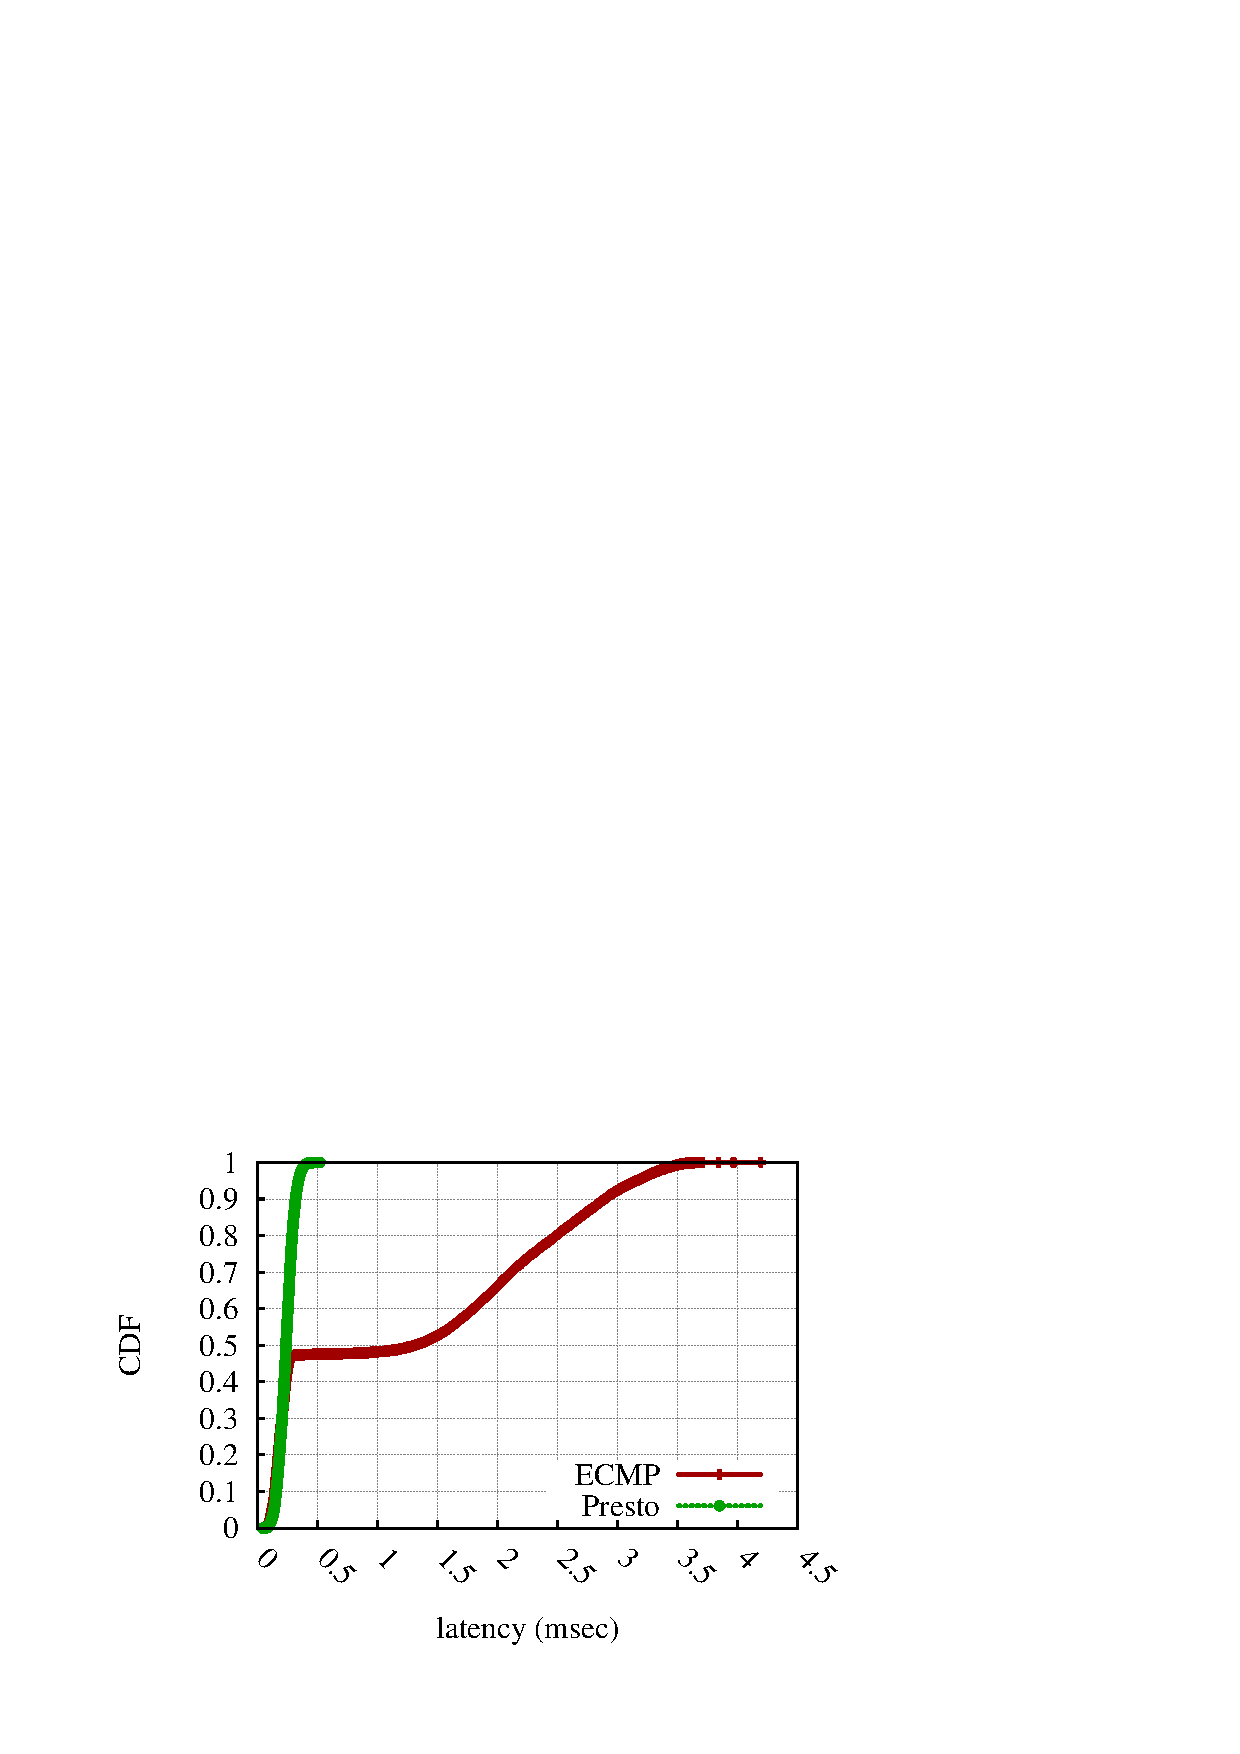
\includegraphics[width=0.45\textwidth]{presto/figures/scalability_test/scalability_compare_latency.pdf}
        \caption{Round trip time comparison in scalability benchmark. 
		%We increase the number of spine switches (i.e., the number of intermediate paths)
                %and set the number of flows (host pairs) equal to the number of available paths. 
		}
        \label{micro_scalability_test_latency}
\end{figure}


\begin{figure}[t]
        \centering
	\centering
        \begin{subfigure}[b]{0.225\textwidth}
                \centering
		\includegraphics[width=\textwidth]{presto/figures/scalability_test/scalability_compare_loss.pdf}
		\caption{}
		\label{micro_scalability_test_loss}
        \end{subfigure}
        \begin{subfigure}[b]{0.225\textwidth}
  		\includegraphics[width=\textwidth]{presto/figures/scalability_test/scalability_compare_fairness.pdf}
        	\caption{}
        	\label{micro_scalability_test_fairness}
	\end{subfigure}
	\caption{(a) Loss rate and (b) Fairness index comparison in scalability benchmark.}
\end{figure}

\tightparagraph{Presto Scales to Multiple Paths}
We analyze Presto's ability to scale in the number of paths by
setting the number of flows (host pairs) equal to the number of available paths in the topology shown in 
Figure~\ref{micro_scalability_topology}. The number of paths is varied from 2 to 8, and 
Presto always load-balances over all available paths.
Figure~\ref{micro_scalability_test_tput} shows Presto's throughput closely tracks Optimal. 
ECMP (and MPTCP) suffer from lower throughput when flows (or subflows) are
hashed to the same path. Hashing on the same path leads to congestion and thus increased latency, as shown in Figure~\ref{micro_scalability_test_latency}.
Because this topology is non-blocking and Presto load-balances in a near optimal fashion, Presto's latency
is near Optimal. Packet drop rates are presented in Figure~\ref{micro_scalability_test_loss} and show
Presto and Optimal have no loss. MPTCP has higher loss because of its bursty nature~\cite{conga}
and its aggression in the face of loss: when a single loss occurs, only
one subflow reduces its rate. The other schemes are more conservative because a single loss reduces the rate of the whole flow.
Finally, Figure~\ref{micro_scalability_test_fairness} shows Presto, Optimal and MPTCP
achieve almost perfect fairness.
%The underlying reason is that MPTCP makes traffic more bursty~\cite{conga}.


%%%congestion test figures %%%%
\begin{figure}[t]
        \centering
  \includegraphics[width=0.45\textwidth]{presto/figures/congestion_test/congestion_compare_tput_witherrbar.pdf}
        \caption{Throughput comparison in oversubscription benchmark.}
        \label{micro_congestion_test_tput}
\end{figure}


\begin{figure}[t]
        \centering
  \includegraphics[width=0.45\textwidth]{presto/figures/congestion_test/congestion_compare_latency.pdf}
        \caption{Round trip time comparison in oversubscription benchmark.
		}
        \label{micro_congestion_test_latency}
\end{figure}



\begin{figure}[t]
        \centering
	\centering
        \begin{subfigure}[b]{0.225\textwidth}
                \centering
		\includegraphics[width=\textwidth]{presto/figures/congestion_test/congestion_compare_loss.pdf}
		\caption{}
		\label{micro_congestion_test_loss}
	\end{subfigure}
	\begin{subfigure}[b]{0.225\textwidth}
		\centering
  		\includegraphics[width=\textwidth]{presto/figures/congestion_test/congestion_compare_fairness.pdf}
		\caption{}
        \label{micro_congestion_test_fairness}
	\end{subfigure}
	\caption{(a) Loss rate and (b) Fairness index comparison in oversubscription benchmark.}
\end{figure}

\tightparagraph{Presto Handles Congestion Gracefully}
Presto's ability to handle congestion is analyzed by fixing 
the number of spine and leaf switches to 2 and varying
the number of flows (host pairs) from 2 to 8, as shown
in Figure~\ref{micro_congestion_topology}. 
Each flow sends as much as possible, which leads to the network
being oversubscribed by a ratio of 1 (two flows) to 4 (eight flows).
Figure~\ref{micro_congestion_test_tput} shows all schemes track Optimal in highly
oversubscribed environments. ECMP
does poorly under moderate congestion because the limited number of flows can be hashed to the same path.
Presto does no worse in terms of latency (Figure~\ref{micro_congestion_test_latency}) and loss (Figure~\ref{micro_congestion_test_loss}).
The long tail latency for MPTCP is caused by its higher loss rates.
Both Presto and MPTCP have greatly improved fairness compared with ECMP (Figure~\ref{micro_congestion_test_fairness}).

\begin{figure}[!t]
        \centering
  \includegraphics[width=0.45\textwidth]{presto/figures/flowlets/flowlet_switching/flowlet_presto_compare_sockperf.pdf}
        \caption{Round trip time comparison of flowlet switching and Presto in Stride workload. 
		The throughputs of Flowlet switching with 100 $\mu\text{s}$ gap, 500 $\mu\text{s}$ gap and Presto 
		are 4.3 Gbps, 7.6 Gbps and 9.3 Gbps respectively. }
        \label{micro_flowlet_rtt_compare}
\end{figure}


\tightparagraph{Comparison to Flowlet Switching}
We first implemented a flowlet load-balancing scheme in OVS that detects
inactivity gaps and then schedules flowlets over disjoint paths in a round robin fashion.
%(Presto does this over flowcells instead of flowlets).
The receiver for flowlets uses official GRO.
Our flowlet scheme is not a direct reflection of CONGA because (i) it is not 
congestion-aware and (ii) the flowlets are determined in the software edge
instead of the networking hardware.
Presto is compared to 500 $\mu$s and 100 $\mu$s inactivity timers in
the stride workload on the 2-tier Clos network (Figure~\ref{macro_evaluation_topology}).
The throughput of the schemes are 9.3 Gbps (Presto), 7.6 Gbps (500 $\mu$s), and 4.3 Gbps (100 $\mu$s).
%Switching flowlets on very small timescales, such as 100$\mu$s, provides opportunities to create many flowlets.
%The largest flowlet is only 0.20\% (XX) of the total network traffic, which corresponds to about 5-9 MB in our runs.
%And while small flowlets create an even distribution
%of traffic over the network, significant strain is put on the TCP connection due to packet reordering. 
Analysis of the 100 $\mu$s
network traces show 13\%-29\% packets in the connection are reordered, which means 100 $\mu$s is not enough
time to allow packets to arrive in-order at the destination and thus throughput is severely impacted. Switching flowlets with 500 $\mu$s prevents
most reordering (only 0.03\%-0.5\% packets are reordered), but creates very large flowlets (see Figure~\ref{micro_flowlet_size}). This means
flowlets can still suffer from collisions, which can hurt throughput (note: while not shown here, 500 $\mu$s outperforms ECMP by over 40\%).
Figure~\ref{micro_flowlet_rtt_compare} shows the
latencies. Flowlet 100 $\mu$s has low throughput and hence lower latencies. However, since
its load balancing isn't perfect, it can still cause increased congestion in the tail. Flowlet 500 $\mu$s
also has larger tail latencies because of more pronounced flowlet collisions. As compared to the flowlet
schemes, Presto decreases 99.9$^{th}$ percentile latency by 2x-3.6x.
%Presto, by enforcing small flowlet sizes and explicitly accounting for reordering on the receiver, can obtain near
%line rate throughput with minimal tail latencies. 



%%%%presto 2 mods (ecmp and shaodw MAC) compare
\begin{figure}[!t]
        \centering
  \includegraphics[width=0.45\textwidth]{presto/figures/presto_compare_2modes/presto_compare_2mods.pdf}
        \caption{Round trip time comparison between Presto + shadow MAC and Presto + ECMP.
		%Compare Presto 2 modes' (Presto over ECMP and Presto over Shadow MAC) performance.
                %Simple 2-tier Clos network with 4 senders and 4 receivers, 4 paths between any host pair.
                %10 seconds per run, 20 runs. Use {\tt nuttcp} to measure throughput. Use {\tt sockperf}
                %to measure latency (RTT).
                %In Presto+ECMP, the average throughput is 7.9 (8.7 if trade latency for tput)
                %Gbps while in Presto+Shadow MAC, the
                %average throughput is 9.3Gbps 
		}
        \label{micro_presto_2mods}
\end{figure}

\tightparagraph{Comparison to Local, Per-Hop Load Balancing}
Presto sends flowcells in a round robin fashion over pre-configured end-to-end paths. An alternative is to
have ECMP hash on flowcell ID and thus provide per-hop load balancing. 
%One way to implement Presto + ECMP is to let vSwitch copy real TCP source port into a pre-allocated TCP option field 
%(\todo{this requires TCP stack allocates the new TCP option before sending to vSwitch}) and 
%encode chunk ID into TCP source port field. Because chunk ID is incremental, ECMP randomly maps chunks into multiple paths. 
We compare Presto + shadow MAC with Presto + ECMP using a stride workload on our testbed. 
Presto + shadow MAC's average throughput is 9.3 Gbps while Presto + ECMP's is 8.9 Gbps.
The round trip time CDF is shown in Figure~\ref{micro_presto_2mods}. 
Presto + shadow MAC gives better latency performance compared with Presto + ECMP. 
The performance difference comes from the fact that Presto + shadow MAC provides 
better fine-grained flowcell load balancing because 
randomization in per-hop multipathing can lead to corner cases where
a large fraction of flowcells get sent to the same link over a small timescale by multiple flows. This transient congestion
can lead to increased buffer occupancy and higher delays.

\section{Evaluation}
\label{sec:eval}

%~\todo{needs to go through the text and make sure they are consistent with the figures!!!}
In this section, we analyze the performance of Presto for (i) synthetic workloads, (ii)
trace-driven workloads, (iii) workloads containing north-south cross traffic, and (iv) failures.
All tests are run on the topology in Figure~\ref{macro_evaluation_topology}.
\begin{figure}[!t]
        \centering
  \includegraphics[width=0.45\textwidth]{./figures/macro/stride/macro_compare_tput_witherrbar.pdf}
        \caption{Elephant flow's throughputs of ECMP, MPTCP, Presto and Optimal in Shuffle, Random, Stride and Random Bijection workloads.}
        \label{macro_evaluation_tput}
\end{figure}



\begin{figure*}[!t]
        \centering
	\begin{subfigure}[b]{0.3\textwidth}
                \centering
  		\includegraphics[width=\textwidth]{./figures/macro/stride/macro_compare_fct_stride_mice.pdf}
        	\caption{Stride}
        	\label{macro_evaluation_fct_stride}
	\end{subfigure}
	\begin{subfigure}[b]{0.3\textwidth}
                \centering
		\includegraphics[width=\textwidth]{./figures/macro/bijection/macro_compare_fct_bijection_mice.pdf}
        	\caption{Random Bijection}
        	\label{macro_evaluation_fct_bijection}
	\end{subfigure}
        %\begin{subfigure}[b]{0.225\textwidth}
        %        \centering
	%	\includegraphics[width=\textwidth]{./figures/macro/random/macro_compare_fct_random_mice.pdf}
        %	\caption{Random}
        %	\label{macro_evaluation_fct_random}
	%\end{subfigure}
        \begin{subfigure}[b]{0.3\textwidth}
                \centering
		\includegraphics[width=\textwidth]{./figures/macro/shuffle/macro_compare_fct_shuffle_mice.pdf}
        	\caption{Shuffle}
        	\label{macro_evaluation_fct_shuffle}
	\end{subfigure}
	\caption{Mice FCT of ECMP, MPTCP, Presto and Optimal in stride, random bijection, and shuffle workloads.}
	\label{macro_evaluation_fct}
\end{figure*}

\tightparagraph{Synthetic Workloads}
Figure~\ref{macro_evaluation_tput} 
shows the average throughputs of elephant flows in the shuffle, random, stride and random bijection workloads.
Presto's throughput is within 1-4\% of Optimal over all workloads.
For the shuffle workload, ECMP, MPTCP, Presto and Optimal show similar results 
because the throughput is mainly bottlenecked at the receiver. 
%due to several servers sending to the same receiver.
In the non-shuffle workloads, Presto improves upon ECMP by 38-72\% and improves
upon MPTCP by 17-28\%.
%Compared with ECMP, 
%Presto improves throughput by 71\% (stride), 72\% (random bijection) and 38\% (random).
%Presto also outperforms MPTCP with throughput improvements of 23\% (stride), 28\% (random bijection) and 
%17\% (random).
%In all the workloads, Presto's throughput outperforms MPTCP.

Figure~\ref{macro_evaluation_fct} shows the mice flow completion time (FCT) in
the workloads. 
The stride and random bijection workloads are non-blocking, and hence the latency of Presto
closely tracks Optimal: the 99.9$^{th}$ percentile FCT for Presto is within 350 $\mu$s for these workloads.
MPTCP and ECMP suffer from congestion, and therefore the tail FCT is much worse than Presto: ECMP's 99.9$^{th}$ percentile
FCT is over 7.5x worse ($\sim$11ms) and MPTCP experiences timeout (because of higher loss
rates and the fact that small sub-flow window sizes from small flows can increase the chances of timeout~\cite{dc-mptcp}).\footnote{We used the Linux default (200ms) and trimmed graphs for clarity}
The difference in the random and shuffle workloads is less pronounced (we omit random due to space constraints).
In these workloads elephant flows can collide on the last hop output port,
and therefore mice FCT is mainly determined by queuing latency. In shuffle, the 99.9$^{th}$ percentile FCT for ECMP, Presto and Optimal
are all within 10\% (MPTCP again experiences TCP timeout) and in random, the 99.9$^{th}$ percentile FCT of Presto is within 25\% of Optimal while ECMP's 
is 32\% worse than Presto.


%%the following are combined into one figure
\iffalse
\begin{figure}[!t]
        \centering
  \includegraphics[width=0.45\textwidth]{./figures/macro/bijection/macro_compare_fct_bijection_mice.pdf}
        \caption{Macro evaluation - flow completiom time in Random Bijection workload}
        \label{macro_evaluation_fct_bijection}
\end{figure}

\begin{figure}[!t]
        \centering
  \includegraphics[width=0.45\textwidth]{./figures/macro/random/macro_compare_fct_random_mice.pdf}
        \caption{Macro evaluation - flow completiom time in Random workload}
        \label{macro_evaluation_fct_random}
\end{figure}


\begin{figure}[!t]
        \centering
  \includegraphics[width=0.45\textwidth]{./figures/macro/shuffle/macro_compare_fct_shuffle_mice.pdf}
        \caption{Macro evaluation - flow completiom time in Shuffle workload}
        \label{macro_evaluation_fct_shuffle}
\end{figure}

\fi

\iffalse
\begin{table}[!htb]
\begin{center}
\begin{tabular}{ |c|c|c|c|c| } 
 \hline
 Shuffle & ECMP & MPTCP & Presto & Optimal \\
 \hline 
 Median & 401 & 874 & 387 & 369  \\ 
 90\%   & 1037 & 2664 & 726 & 712 \\
 99\%   & 3373 & 21600  & 2447 & 2446 \\ 
 99.9\% & 12830 & 206ms & 12480 & 11714 \\
 %99.99\% & 204.1ms & - & 204.1ms & 203.6ms \\
 \hline

\end{tabular}
\caption{Macro evaluation - A close look of flow completiom time in Shuffle workload}
        \label{macro_evaluation_fct_shuffle_closelook}
\end{center}
\end{table}

\begin{table}[!htb]
\begin{center}
\begin{tabular}{ |c|c|c|c|c| }
 \hline
 Random & ECMP & MPTCP & Presto & Optimal \\
 \hline
 Median & 1008 & 780 & 648 & 595  \\
 90\%   & 3815 & 1918 & 2850 & 2297 \\
 99\%   & 7852 & 3380  & 6900 & 4936 \\
 99.9\% & 11784 & 202ms & 9372 & 7127 \\
% 99.99\% & 11677 & - & 16591 & 200ms \\
 \hline

\end{tabular}
\caption{Macro evaluation - A close look of flow completiom time in Random workload}
        \label{macro_evaluation_fct_random_closelook}
\end{center}
\end{table}

\fi

%%% trace-driven workload, MSR, scaling factor =10
\begin{table}[!tb]
\begin{center}
\begin{tabular}{ |c|c|c|c| }
 \hline
 Percentile & ECMP & Optimal &Presto \\
 \hline
 50\%   & $1.0$ & $-12\%$ & $-9\%$   \\
 90\%   & $1.0$ & $-34\%$ & $-32\%$  \\
 99\%   & $1.0$ & $-63\%$  & $-56\%$ \\
 99.9\% & $1.0$ & $-61\%$ & $-60\%$  \\
 \hline

\end{tabular}
\caption{Mice ($<$100KB) FCT in trace-driven workload~\cite{kandula2009nature}. Negative numbers imply shorter FCT.}
        \label{macro_evaluation_MSR_trace_driven}
\end{center}
\end{table}

\tightparagraph{Trace-driven Workload}
We evaluate Presto using a trace-driven workload based on traffic patterns measured in~\cite{kandula2009nature}. 
Each server establishes a long-lived TCP connection 
with every other server in the testbed. 
Then each server continuously samples flow sizes and inter-arrival times and each time sends to a random receiver
that is not in the same rack.
%Since 99\% of flows are less than 4MB in the distribution, 
We scale the flow size distribution by a factor of 10 to emulate a heavier workload. 
Mice flows are defined as flows that are less than 100 KB in size, and elephant flows are defined as flows
that are greater than 1 MB. The mice FCT, normalized to ECMP, 
is shown in Table~\ref{macro_evaluation_MSR_trace_driven}. 
Compared with ECMP, Presto has similar performance at the 50$^{th}$ percentile but reduces the 99$^{th}$ and 99.9$^{th}$ percentile FCT by 56\% and 60\%, respectively. 
Note MPTCP is omitted because its performance was quite unstable in workloads
featuring a large number of small flows.
The average throughput (not shown) for Presto tracks Optimal (within 2\%), and improves upon ECMP by over 10\%.


\begin{table}[!htb]
\begin{center}
\begin{tabular}{ |c|c|c|c|c| }
 \hline
% Percentile & 50\% & 90\% & 99\% & 99.9\% \\
% \hline
% ECMP & 1.0 & 1.0 & 1.0 & 1.0  \\
% N-block   & 66\% & 17\% & 11\% & 9\% \\
% Presto    & 80\% & 21\% & 14\% & 10\% \\
% MPTCP     & 88\% & 27\% & 27\% & TIMEOUT \\

 Percentile & ECMP & Optimal & Presto & MPTCP \\
 \hline
 50\%       & 1.0 & $-34$\%     & $-20$\%   & $-12$\% \\
 90\%       & 1.0 & $-83$\%     & $-79$\%   & $-73$\% \\
 99\%       & 1.0 & $-89$\%     & $-86$\%   & $-73$\% \\
 99.9\%     & 1.0 & $-91$\%      & $-87$\%   & TIMEOUT \\

 \hline
\end{tabular}
\caption{FCT comparison (normalized to ECMP) with ECMP load balanced north-south traffic.}
	\label{macro_evaluation_north_south_traffic}
\end{center}
\end{table}


\tightparagraph{Impact of North-South Cross Traffic}
Presto load balances on "east-west" traffic in the datacenter, \ie{}, traffic
originating and ending at servers in the datacenter. 
In a real datacenter environment "north-south" traffic (\ie{}, traffic with an endpoint outside the datacenter)
must also be considered. 
%Ideally, north-south traffic should be load balanced by ECMP because of 
%reordering concerns at the end user. 
%However, east-west traffic typically dominates (75\% according to~\cite{east-west}). 
To study the impact of north-south traffic on Presto, we attach an additional server to 
each spine switch in our testbed to emulate remote users. 
The 16 servers establish a long-lived TCP connection with each remote user. 
Next, each server starts a flow to a random remote user every 1 millisecond. This emulates  
the behavior of using ECMP to load balance north-south traffic.
The flow sizes for north-south traffic are based on the distribution measurement in~\cite{he2013next}. 
The throughput to remote users is limited to 100Mbps to emulate the limitation of an Internet WAN. 
Along with the north-south flows, 
a stride workload is started to emulate the east-west traffic. 
The east-west mice FCT is shown in Table~\ref{macro_evaluation_north_south_traffic} (normalized to ECMP). 
ECMP, MPTCP, Presto, and Optimal's average throughput is 
5.7, 7.4, 8.2, and 8.9Gbps respectively. 
The experiment shows Presto can gracefully co-exist with north-south cross traffic
in the datacenter.


%%%failure handling experiments

\begin{figure}[t]
        \centering
  \includegraphics[width=0.45\textwidth]{./figures/failure_handling/failover_compare_tput_witherrbar.pdf}
        \caption{Presto's throughput in symmetry, fast failover and weighted multipathing stages for different workloads.}
        \label{failover_compare_tput}
\end{figure}

\begin{figure}[t]
        \centering
  \includegraphics[width=0.45\textwidth]{./figures/failure_handling/failover_compare_sockperf_bijection_mice.pdf}
        \caption{Presto's RTT in symmetry, fast failover and weighted multipathing stages in  random bijection workload.}
        \label{failover_compare_sockperf_bijection}
\end{figure}

\tightparagraph{Impact of Link Failure}
Finally, we study the impact of link failure.
Figure~\ref{failover_compare_tput} compares the throughputs of
Presto when %under different stages of loss recovery when 
the link between spine switch S1 and leaf switch L1 goes down.
Three stages are defined: symmetry (the link is up), failover (hardware fast-failover moves traffic from S1 to S2), and weighted (the controller
learns of the failure and prunes the tree with the bad link).
Despite the asymmetry in the topology, Presto still achieves reasonable average throughput at 
each stage.
Figure~\ref{failover_compare_sockperf_bijection} shows the round trip time of
each stage in a random bijection workload. 
Workload L1->L4 is when each node connected to L1 sends to one node in L4 (L4->L1 is the opposite).
Due to the fact that the network is no longer non-blocking after the link failure,
failover and weighted multipathing stages have larger round trip time.



\iffalse
\begin{enumerate}
\item Clos-network, macro. ECMP, MPTCP, Presto and Optimal.
\begin{enumerate}
	\item Workloads: Take from Planck and Hedera. Can do MSR trace-based.
	\item Throughput, fairness, latency (maybe loss). Link utilization?
\end{enumerate}

\item Fat tree, macro. ECMP, MPTCP, Presto and Optimal.
\begin{enumerate}
        \item Workloads: Take from Planck and Hedera. Can do MSR trace-based.
        \item Throughput, fairness, latency (maybe loss). Link utilization?
\end{enumerate}


\item Vary flow sizes. Idea is that we can work on very small elephants.

\item Failure: backbone switch fails, aggregate switch fails, ToR switch fails, link fails, ...

\item CONGA uses incast, should we check?

\item Maybe this belongs in micro: ECMP vs shadowMAC for multipathing.

\end{enumerate}
\fi

\section{Related Work}
\label{related}
This section discusses different classes of related work.

\tightparagraph{Congestion control for DCNs}
\crs{Rather than proposing a new congestion control algorithm, our work investigates if congestion control can be moved to the vSwitch.
Thus, many of the following schemes are complimentary.}
DCTCP~\cite{dctcp} is a seminal TCP variant for datacenter networks.
Judd~\cite{judd2015nsdi} proposed simple yet practical fixes to enable DCTCP in production networks.
TCP-Bolt~\cite{stephens2014practical} is a variant of DCTCP for PFC-enabled lossless Ethernet.
%DCQCN~\cite{zhu2015congestion} is a rate-based congestion control scheme implemented in NICs
%for QCN-based~\cite{qcn} RDMA deployments.
DCQCN~\cite{zhu2015congestion} is a rate-based congestion control scheme (built on DCTCP and QCN) to
support RDMA deployments in PFC-enabled lossless networks.
TIMELY~\cite{mittal2015timely} and DX~\cite{lee2015accurate} 
use accurate network latency as the signal to perform congestion control.
TCP ex Machina~\cite{winstein2013tcp} uses computer-generated congestion control rules.
PERC~\cite{jose2015high} proposes proactive congestion control to improve convergence.
ICTCP's~\cite{wu2010ictcp} receiver monitors incoming TCP flows and 
modifies~\rwnd{} to mitigate the impact of incast, but this cannot
provide generalized congestion control like~\acdc{}.
Finally, efforts~\cite{dell-toe,chelsio-toe} to 
implement TCP Offload Engine (TOE) in specialized NICs are not widely deployed for reasons noted in~\cite{mogul2003tcp,linux-toe}.
%~\acdc{} is designed to work with commodity NICs. 

\tightparagraph{Bandwidth allocation} Many bandwidth allocation schemes have been proposed.
Gatekeeper~\cite{rodrigues2011gatekeeper} and EyeQ~\cite{jeyakumar2013eyeq} abstract the network as a single
switch and provide bandwidth guarantees by managing each server's access link.
Oktopus~\cite{Ballani2011oktopus} provides fixed performance guarantees within virtual clusters.
SecondNet~\cite{Guo2010Secondnet} enables virtual datacenters with static bandwidth guarantees.
Proteus~\cite{Xie2012Proteus} allocates bandwidth for applications with dynamic demands.
Seawall~\cite{shieh2011sharing} provides bandwidth proportional to a defined weight by
forcing traffic through congestion-based edge-to-edge tunnels. 
NetShare~\cite{Lam2012NetShare} utilizes hierarchical weighted max-min fair sharing to tune relative bandwidth allocation for services.
FairCloud~\cite{Popa2012Faircloud} identifies trade-offs in minimum
guarantees, proportionality and high utilization, and designs schemes over this space.
Silo~\cite{jang2015silo} provides guaranteed bandwidth, delay and burst allowances through a novel VM placement and admission 
algorithm, coupled with a fine-grained packet pacer. As discussed in~\sref{background}, 
~\acdc{} is largely complimentary to these schemes because it is a transport-level solution.

\tightparagraph{Rate limiters} 
SENIC~\cite{niranjan2013fastrak} 
identifies the limitations of NIC hardware rate limiters (\ie{}not scalable) and 
software rate limiters (\ie{}high CPU overhead) and uses the CPU to enqueue packets 
in host memory and the NIC. Silo's pacer injects void packets into 
an original packet sequence to achieve pacing. FasTrack~\cite{niranjan2013fastrak} offloads
functionality from the server into the switch for certain flows.~\acdc{} prevents
TCP flows from sending in the first place and can be used in conjunction with these
schemes.


\tightparagraph{Low latency DCNs}
Many schemes have been proposed to reduce latency in datacenter networks.
HULL~\cite{alizadeh2012less} uses phantom queues to leave bandwidth headroom to support low latency.
pFabric~\cite{alizadeh2013pfabric} is a clean-slate
design which utilizes priority and minimal switch buffering to achieve low latency.
Fastpass~\cite{perry2014fastpass} uses a centralized arbiter to
perform per-packet level scheduling.
QJUMP~\cite{qjump} uses priority queueing and rate limiting to
bound latency. Traffic engineering~\cite{hedera,rasley2014planck} and 
load balancing~\cite{conga,he2015presto,ghorbani2015micro} can also
reduce latency. Because~\acdc{} works on the transport level, it is
largely complimentary to these works.

\tightparagraph{Performance-enhancing proxies}
Several schemes improve end-to-end protocol performance via a middlebox
or proxy~\cite{RFC3449,RFC3115,balakrishnan2008maelstrom,davern2011httpep,balakrishnan1995improving}.
\acdc{} fits into this class of works, but is unique in providing a mechanism
to alter a VM's TCP congestion control algorithm by modifying the vSwitch.

\tightparagraph{Virtualized congestion control}
\crs{vCC~\cite{vcc} is a concurrently designed system that shares~\acdc{}'s goals and some of its design details.
The paper is complementary in that some items not addressed in this work are presented, such as a more detailed
analysis of the ECN-coexistence problem, an exploration of the design space, and a theoretical proof of
virtualized congestion control's correctness. Our paper provides an in-depth design and thorough evaluation of
a DCTCP-based virtualized congestion control algorithm on a 10 Gbps testbed.
}

%\section{Discussion}
\label{discuss}

\tightparagraph{UDP traffic} How to handle. 
Mention VxLAN traffic too.
\keqiang{and IPsec}

\tightparagraph{No vSwitch} 
\keqiang{title should be hypervisor-bypass?}
Use middleboxes (for DB server).
Use NIC (for SR-IOV).
Hypervisor bypass (e.g., SR-IOV), where TCP traffic is sent to the NIC directly without 
going through hypervisor. First, as noted by~\cite{shieh2011sharing}, ``loss of the security and 
manageability features provided by the software virtual switch has limited 
the deployment of direct I/O NICs in public clouds''. Second, based on techniques like Intel 
DPDK~\cite{intel-dpdk} and ``smart NICs''~\cite{cavium-nic,netronome-nic}, we believe that low latency 
congestion control enforcement schemes like \acdc{} can also be 
employed for hypervisor bypass use cases.
We need to worry about legacy systems and non-VM systems. For instance, a database or storage device that may not have OVS installed on it.
We need to talk about either a middlebox or that this percentage of traffic is low? Or implement in NIC (especially one with OVS offload?).

\tightparagraph{North-South traffic.}
Transport enforcement should be only be done for east west traffic, so if the tenant tuned their stack's
congestion control algorithm for wide-area networks, their north sourth traffic is not affected and their 
congestion control scheme can still achieve good performance.

\keqiang{todos: some figures do not read well on printed paper}
\keqiang{todos: sometimes, when we refer a section, we say ``Section X'', sometimes, we use the 
dollar sign, we should unify them}

%
%Byzantine VM.
%
%Other names: ACDCTCP, LiquidSwitch, LiquidEdge
%
%In CPU overhead measurement, we need to 
%mention ovs add 1 widecard rule. That means we isolated the overhead of 
%OVS itself when it has many flows in its flow table (probably it does not matter
%at the end of the day, because we measured the CPU usage of the whole system).
%
%People may say window-based congestion control is burty. TIMELY operates 
%on TCP segments in order to reduce CPU overhead. Therefore, TIMELY is also
%busty. In TIMELY, they mentioned they can leverage a hybrid scheme, that is
%using software to control large segments and use hardware rate limiter to
%reduce burstyness.
%
%Create loss and check how DCTCP and our scheme treates packet losses (revisit it after we finish incast 
%and macrobenchmarks).
%
%One more microbenchmark on the Dumbbell topology: different servers have different transport, so the
%throughput fairness among different transports (e.g., start cubic, start New Reno, start dctcp).
%
%A point that is missing in DCTCP and NSDI paper is that they did not mention how the switch should be
%configured to handle non-TCP traffic. Note non-TCP traffic such as DNS (UDP 53) and ARP, ICMP etc
%are also important. We found that if we did not specify how the switch handle the non-TCP traffic,
%then this kind of non-TCP traffic can be easily dropped by the switch. We found ARP traffic is dropped
%by the switch such that DCTCP flows stall. Hence, we think it is better to put non-TCP traffic
%into a different queue when we apply WRED/ECN on the switches.
%
%This work offers low latency for ``hetergeneous networks" where different entities can 
%run different kinds of
%transport congestion control schemes. A few examples of such hetergeneous networks: public 
%datacenters where tenants can set up their own VMs (e.g., AWS), or tenants can rent their bare metal
%machines (e.g., SoftLayer), or certain groups (even within a single organization) 
%have to use traditional transports due to compatibility of legacy applications (NSDI's Judd said this), or
%incremental deployment is undergoing. 
%To ensure a pure low latency datacenter network, a universal transport enforcement scheme is required. 
%Two challenges to implement such a transport enforcement scheme are scalability and low overhead. 
%The transport enformancement scheme proposed here meet the two metrics (as shown in our experiments) while
%providing nice network performance (throughput, latency and packet drop rate). This scheme is 
%compatible with any kind of TCP stack. Finally, the scheme we propose solves the co-existence issue of 
%ECT (ECN Capable Transport) and non-ECT, which is a critical deployment hurdle for DCTCP-like transports.
%
%Macrobenchmark plan: 18 hosts, 6 switches, ECMP configured. The network oversubscription ratio is 2:1.
%Run all-to-all traffic for a long time (e.g., 1 hours). Show total throughput and TCP RTT and packet drop 
%rate.
%
%QoS can be implemented too?
%
%
%
%When we try to launch an instance in EC2: ``An AMI is a template that contains the software 
%configuration (operating system, application server, and applications) required to launch your instance. 
%You can select an AMI provided by AWS, our user community, or the AWS Marketplace; 
%or you can select one of your own AMIs''. Default is CUBIC for most Linux images, Window Servers can
%have NewReno, Compound TCP (CTCP)~\cite{tan2006compound} and DCTCP. 
%Users can tweak congestion control algorithms to optimize network performance for their target scenarios. 
%
%Section talking about how to implement other CC schemes: TIMELY, PERC, Vegas, etc.
%
%EJR: VXLAN, UDP, TCP stack statistics for Cloud?
%
%ECT and non-ECT: througput unfairness, long RTT, connection establishment..
%
%
%EyeQ, Seawall, NetShare, Silo, SecondNet, Oktopus etc. Our work did not provide bandwidth allocation property. 
%This work focused on reducing in-network queuing latency caused by VM TCP stacks. 
%We show how this goal can be done using a simple and elegant solution.
%Yes, if an VM opens more connections than another, that VM gains more bandwidth. 
%But, there are proposals which try to provide proper bandwidth allocation when multiple end-points compete 
%at the sender side or receiver side. Those works and this work are complementary. 
%To the best of our knowledge, today's cloud providers have not provide strong bandwidth guarantees 
%(for example, AWS only roughly classify VMs instances' network performance into 
%``low to moderate", ``moderate", ``high" and ``10 Gigabit"categories).
%
%talk about containers?

\section{Summary} 
\label{rate-limiter:sec:conclusion} 

A lot of recent work has been focusing on solving in network latency in datacenter networks.
In this paper, we focus on a less explored topic \textemdash\xspace latency
increase caused by rate limiters on the end-host.
We show that latency can be increased by an order of magnitude
by the rate limiters in cloud networks,
and simply extending ECN into rate limiters is not sufficient.
To this end, we propose two techniques \textemdash\xspace~\dem{} and~\spring{} to improve the performance of rate limiters.
Our experiment results demonstrate that~\dem{} and~\spring{} enabled
rate limiters can achieve high (and stable) throughput and low latency.


{\scriptsize
\setlength{\bibsep}{0.5pt}
\raggedright
\bibliographystyle{abbrv}
\bibliography{refer}
}

\end{document}
